\documentclass{beamer}
\usepackage[utf8]{inputenc}

\usetheme{Madrid}
\usecolortheme{default}
\usepackage{amsmath,amssymb,amsfonts,amsthm}
\usepackage{txfonts}
\usepackage{tkz-euclide}
\usepackage{listings}
\usepackage{adjustbox}
\usepackage{array}
\usepackage{tabularx}
\usepackage{gvv}
\usepackage{lmodern}
\usepackage{circuitikz}
\usepackage{tikz}
\usepackage{graphicx}

\setbeamertemplate{page number in head/foot}[totalframenumber]

\usepackage{tcolorbox}
\tcbuselibrary{minted,breakable,xparse,skins}



\definecolor{bg}{gray}{0.95}
\DeclareTCBListing{mintedbox}{O{}m!O{}}{%
  breakable=true,
  listing engine=minted,
  listing only,
  minted language=#2,
  minted style=default,
  minted options={%
    linenos,
    gobble=0,
    breaklines=true,
    breakafter=,,
    fontsize=\small,
    numbersep=8pt,
    #1},
  boxsep=0pt,
  left skip=0pt,
  right skip=0pt,
  left=25pt,
  right=0pt,
  top=3pt,
  bottom=3pt,
  arc=5pt,
  leftrule=0pt,
  rightrule=0pt,
  bottomrule=2pt,

  colback=bg,
  colframe=orange!70,
  enhanced,
  overlay={%
    \begin{tcbclipinterior}
    \fill[orange!20!white] (frame.south west) rectangle ([xshift=20pt]frame.north west);
    \end{tcbclipinterior}},
  #3,
}
\lstset{
    language=C,
    basicstyle=\ttfamily\small,
    keywordstyle=\color{blue},
    stringstyle=\color{orange},
    commentstyle=\color{green!60!black},
    numbers=left,
    numberstyle=\tiny\color{gray},
    breaklines=true,
    showstringspaces=false,
}
%------------------------------------------------------------
%This block of code defines the information to appear in the
%Title page
\title %optional
{4.3.16}
\date{september 2025}
%\subtitle{A short story}

\author % (optional)
{J.NAVYASRI- EE25BTECH11028}

\begin{document}

\frame{\titlepage}
\begin{frame}{Question:}
Find the equation of the plane through the points  
\[
(2,1,0), \quad (3,-2,-2), \quad (3,1,7).
\]
\end{frame}

\begin{frame}{Soultion:}
Let $\mathbf{p}_1, \mathbf{p}_2, \mathbf{p}_3$ be the given points and $\mathbf{x} = \begin{pmatrix} x\\y\\z \end{pmatrix}$ be a general point on the plane. The points are:
\[
\mathbf{p}_1 = \begin{pmatrix} 2\\1\\0 \end{pmatrix}, \quad
\mathbf{p}_2 = \begin{pmatrix} 3\\-2\\-2 \end{pmatrix}, \quad % Corrected P_2: (3, -2, -2)
\mathbf{p}_3 = \begin{pmatrix} 3\\1\\7 \end{pmatrix}.
\]
\end{frame}

\begin{frame}{Soultion:}
\subsection*{Step 1: General Plane Equation}
The equation of the plane is $\mathbf{n} \cdot \mathbf{x} + d = 0$, where $\mathbf{n} = \begin{pmatrix} a\\b\\c \end{pmatrix}$ is the normal vector.
\[
ax + by + cz + d = 0 \tag{1}
\]
\subsection*{Step 2: Substitution of Points}
The points $\mathbf{p}_i$ must satisfy the plane equation:
\end{frame}

\begin{frame}{Soultion:}
\[
2a + b + d = 0 \tag{2}
\]
\[
3a - 2b - 2c + d = 0 \tag{3}
\]
\[
3a + b + 7c + d = 0 \tag{4}
\]
\subsection*{Step 3: Matrix Form}
The system of linear equations can be written as $M \mathbf{v} = \mathbf{0}$, where $\mathbf{v} = \begin{pmatrix} a\\ b\\ c\\ d \end{pmatrix}$:
\[
\begin{pmatrix}
2 & 1 & 0 & 1\\
3 & -2 & -2 & 1\\
3 & 1 & 7 & 1
\end{pmatrix}
\begin{pmatrix} a\\ b\\ c\\ d \end{pmatrix}
=
\begin{pmatrix} 0\\0\\0 \end{pmatrix}
\tag{5}
\]
\end{frame}

\begin{frame}{Soultion:}
\subsection*{Step 4: Solving the System}
From (2):
\[
d = -2a - b \tag{6}
\]

Substitute (6) in (3):
\[
3a - 2b - 2c + (-2a - b) = 0 \;\;\Rightarrow\;\; a - 3b - 2c = 0 \tag{7}
\]

Substitute (6) in (4):
\[
3a + b + 7c + (-2a - b) = 0 \;\;\Rightarrow\;\; a + 7c = 0 \tag{8}
\]
\end{frame}

\begin{frame}{Soultion:}
From (8):
\[
a = -7c \tag{9}
\]

From (7), substitute (9):
\[
(-7c) - 3b - 2c = 0 \;\;\Rightarrow\;\; -9c = 3b \;\;\Rightarrow\;\; b = -3c \tag{10}
\]

From (6), substitute (9) and (10):
\[
d = -2(-7c) - (-3c) = 14c + 3c \;\;\Rightarrow\;\; d = 17c \tag{11}
\]
\end{frame}

\begin{frame}{Soultion:}
\subsection*{Step 5: Final Result}
The coefficient vector $\mathbf{v}$ is proportional to $c$:
\[
\mathbf{v} = \begin{pmatrix} a\\ b\\ c\\ d \end{pmatrix} = c \begin{pmatrix} -7\\ -3\\ 1\\ 17 \end{pmatrix}
\]

Choosing $c=1$, the normal vector is $\mathbf{n} = \begin{pmatrix} -7\\ -3\\ 1 \end{pmatrix}$ and $d=17$. The plane equation is:
\[
-7x - 3y + z + 17 = 0 \tag{12}
\]

Or equivalently, multiplying by $-1$:
\[
\boxed{7x + 3y - z - 17 = 0} \tag{13}
\]
\end{frame}

\begin{frame}[fragile]
\frametitle{Python Code}

\begin{lstlisting}
import numpy as np
import matplotlib.pyplot as plt
from mpl_toolkits.mplot3d import Axes3D

# Given points
P1 = np.array([2, 1, 0])
P2 = np.array([3, -2, -2])
P3 = np.array([3, 1, 7])
\end{lstlisting}

\end{frame}
\begin{frame}[fragile]
\frametitle{Python  Code}

\begin{lstlisting}
# Create a meshgrid for x, y
xx, yy = np.meshgrid(range(-2, 6), range(-3, 6))

# Equation of plane: 7x + 3y - z - 17 = 0  => z = 7x + 3y - 17
zz = 7*xx + 3*yy - 17

# Plot
fig = plt.figure(figsize=(8,6))
ax = fig.add_subplot(111, projection='3d')

# Plot the surface (plane)
ax.plot_surface(xx, yy, zz, alpha=0.5, color='cyan')

# Plot points
ax.scatter(*P1, color='r', s=50, label='P1 (2,1,0)')
ax.scatter(*P2, color='g', s=50, label='P2 (3,-2,-2)')
ax.scatter(*P3, color='b', s=50, label='P3 (3,1,7)')
\end{lstlisting}

\end{frame}
\begin{frame}[fragile]
\frametitle{Python Code}

\begin{lstlisting}
# Labels
ax.set_xlabel('X-axis')
ax.set_ylabel('Y-axis')
ax.set_zlabel('Z-axis')
ax.set_title("Plane: 7x + 3y - z - 17 = 0")

ax.legend()
plt.savefig("fig6.png")
plt.show()

\end{lstlisting}

\end{frame}
\begin{frame}{Plot-Using by Python}
    \centering
    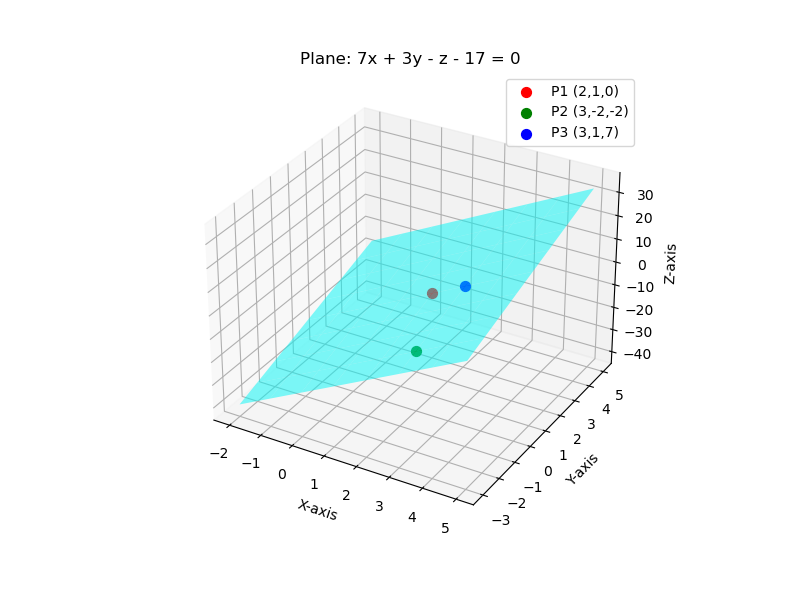
\includegraphics[width=\columnwidth, height=0.8\textheight, keepaspectratio]{figs/fig6.png}     
\end{frame}


\begin{frame}[fragile]
\frametitle{C Code}
\begin{lstlisting}
#include <stdio.h>

// Function to compute gcd
int gcd(int a, int b) {
    if (b == 0) return a > 0 ? a : -a;
    return gcd(b, a % b);
}

// Function to compute gcd of 4 numbers
int gcd4(int a, int b, int c, int d) {
    int g = gcd(a, b);
    g = gcd(g, c);
    g = gcd(g, d);
    return g;
}
\end{lstlisting}

\end{frame}

\begin{frame}[fragile]
\frametitle{C Code}
\begin{lstlisting}
int main() {
    // Given three points
    int x1 = 2, y1 = 1, z1 = 0;
    int x2 = 3, y2 = -2, z2 = -2;
    int x3 = 3, y3 = 1, z3 = 7;
\end{lstlisting}

\end{frame}

\begin{frame}[fragile]
\frametitle{C Code}
\begin{lstlisting}
// Direction vectors
    int v1x = x2 - x1, v1y = y2 - y1, v1z = z2 - z1;
    int v2x = x3 - x1, v2y = y3 - y1, v2z = z3 - z1;

    // Cross product → normal vector (a, b, c)
    int a = v1y * v2z - v1z * v2y;
    int b = v1z * v2x - v1x * v2z;
    int c = v1x * v2y - v1y * v2x;

    // Constant term d
    int d = -(a * x1 + b * y1 + c * z1);

\end{lstlisting}

\end{frame}

\begin{frame}[fragile]
\frametitle{C Code}
\begin{lstlisting}
// Simplify using gcd
    int g = gcd4(a, b, c, d);
    a /= g; b /= g; c /= g; d /= g;

    // Make leading coefficient positive
    if (a < 0) {
        a = -a; b = -b; c = -c; d = -d;
    }

    // Final output
    printf("The equation of plane is: %dx + %dy + %dz + %d = 0\n", a, b, c, d);

    return 0;
}

\end{lstlisting}

\end{frame}


\begin{frame}[fragile]
\frametitle{Python and C Code}

\begin{lstlisting}
import ctypes
import numpy as np
import matplotlib.pyplot as plt
from mpl_toolkits.mplot3d import Axes3D

# Load the compiled C library
lib = ctypes.CDLL("./plane.so")

# Define the cross_product function signature
lib.cross_product.argtypes = [ctypes.POINTER(ctypes.c_double),
                              ctypes.POINTER(ctypes.c_double),
                              ctypes.POINTER(ctypes.c_double)]

# Points
P1 = np.array([2,1,0], dtype=np.double)
P2 = np.array([3,-2,-2], dtype=np.double)
P3 = np.array([3,1,7], dtype=np.double)
\end{lstlisting}

\end{frame}
\begin{frame}[fragile]
\frametitle{Python and C Code}

\begin{lstlisting}
# Direction vectors
v1 = P2 - P1
v2 = P3 - P1

# Prepare ctypes arrays
v1_c = (ctypes.c_double * 3)(*v1)
v2_c = (ctypes.c_double * 3)(*v2)
n_c = (ctypes.c_double * 3)()

# Call C function
lib.cross_product(v1_c, v2_c, n_c)

# Normal vector from C
n = np.array([n_c[0], n_c[1], n_c[2]])
print("Normal vector from C:", n)

# Equation of plane: n·(X - P1) = 0  →  ax+by+cz+d=0
a, b, c = n
d = -(a*P1[0] + b*P1[1] + c*P1[2])
\end{lstlisting}

\end{frame}
\begin{frame}[fragile]
\frametitle{Python and C Code}

\begin{lstlisting}
print(f"Plane equation: {a}x + {b}y + {c}z + {d} = 0")

# ----- Plot -----
fig = plt.figure()
ax = fig.add_subplot(111, projection='3d')

# Plot points
ax.scatter(*P1, color='red', s=50, label="P1(2,1,0)")
ax.scatter(*P2, color='blue', s=50, label="P2(3,-2,-2)")
ax.scatter(*P3, color='green', s=50, label="P3(3,1,7)")
\end{lstlisting}

\end{frame}
\begin{frame}[fragile]
\frametitle{Python and C Code}

\begin{lstlisting}
# Create grid for plane
xx, yy = np.meshgrid(range(0,6), range(-3,3))
zz = (-a*xx - b*yy - d)/c

ax.plot_surface(xx, yy, zz, alpha=0.3, color='yellow')

ax.set_xlabel("X")
ax.set_ylabel("Y")
ax.set_zlabel("Z")
ax.legend()
plt.show()
\end{lstlisting}

\end{frame}

\begin{frame}{Plot-Using by C and Python}
    \centering
    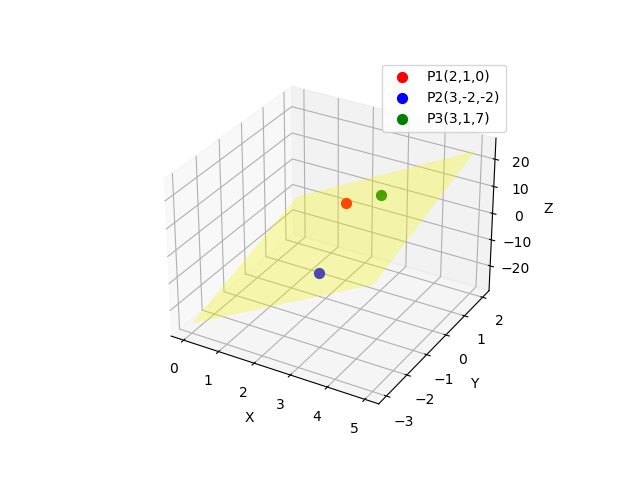
\includegraphics[width=\columnwidth, height=0.8\textheight, keepaspectratio]{figs/fig6.1.png}     
\end{frame}

\end{document}